\section{Dataset}
\setcounter{footnote}{1}

\begin{frame}{Dataset}
    \begin{itemize}
        \item MIT Supercloud Dataset \footnotetext{https://www.kaggle.com/datasets/skylarkphantom/mit-datacenter-challenge-data}
        \item One-year HPC task record
        \item Concerning features: \texttt{time\_submit}, \texttt{time\_start}, \texttt{time\_end}, \texttt{nodes\_alloc}
    \end{itemize}
\end{frame}

\begin{frame}{Dataset Processing}
    \begin{itemize}
        \item Assumption: all nodes have the same computing capacity
        \item Introduce $\texttt{task\_complexity} = (\texttt{time\_end} - \texttt{time\_start}) \times \texttt{nodes\_alloc}$
        \item Train and test data contain \texttt{time\_submit} and \texttt{task\_complexity}.
        \item Due to computation limit, secondly and minutely predictions are intractable. Daily prediction cannot capture patterns. As an experiment, we group complexities by hour.
        \item Dataset is split into $90\%$ for training and $10\%$ for testing.
    \end{itemize}
\end{frame}

\begin{frame}{Dataset Processing}
    \begin{figure}
        \centering
        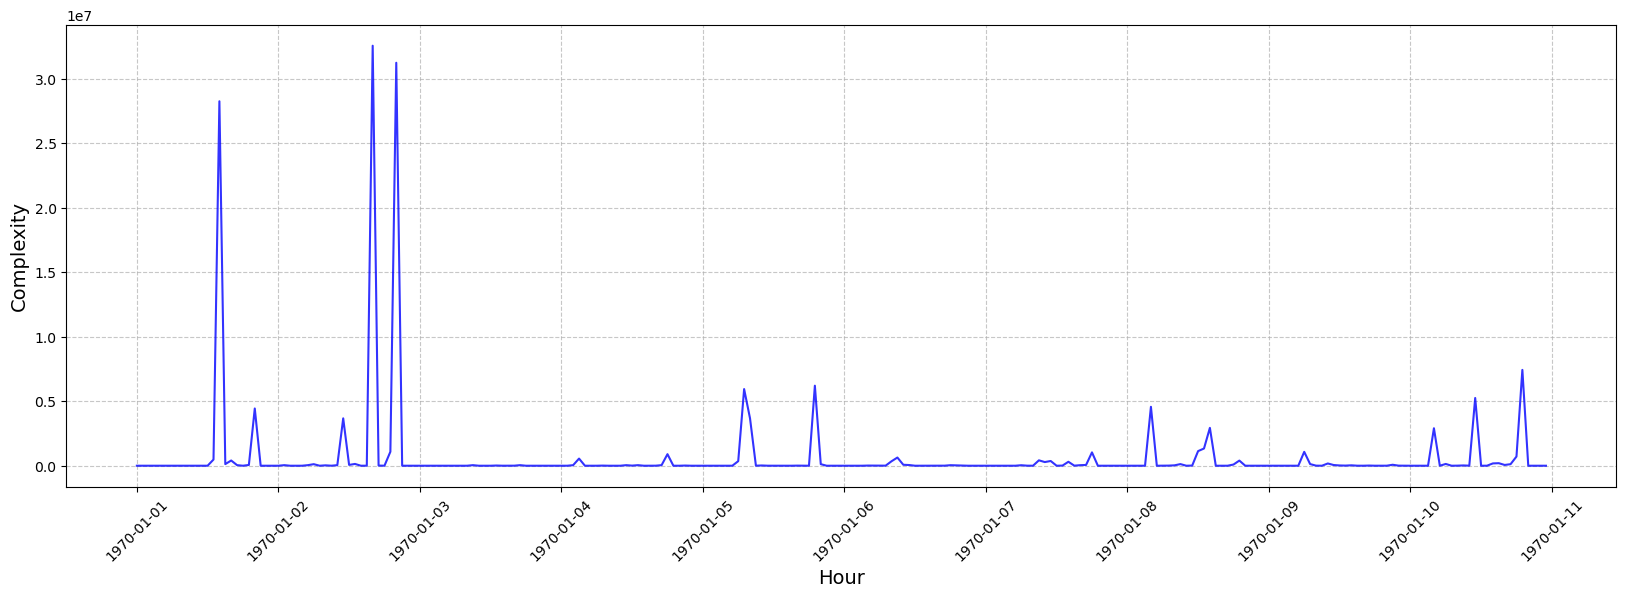
\includegraphics[width=0.8\linewidth]{img/hourly_complexity.png}
        \caption{Task complexity grouped by hour}
    \end{figure}
\end{frame}

\begin{frame}{Dataset Processing}
    \begin{figure}
        \centering
        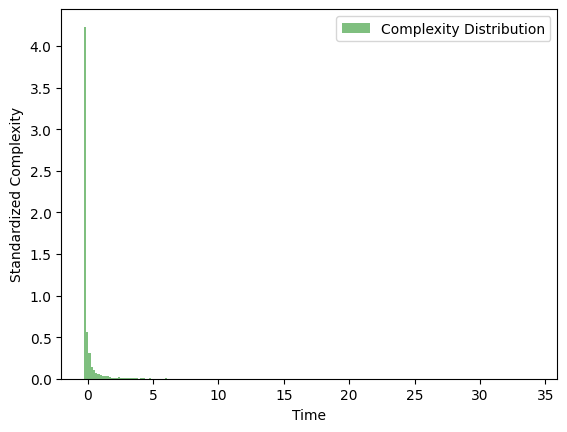
\includegraphics[width=0.7\linewidth]{img/task_complexity_distribution.png}
        \caption{High skewness of task complexity distribution}
    \end{figure}
\end{frame}

